\subsection{流域系统稳态转换的理论框架}

% 宋嘉熙 的 地理学报
本研究对流域系统人-水关系状态的分析植根于社会-生态系统的“稳态”概念,属于生态系统与社会-生态系统研究中,以弹性(Resilience,也被译为韧性)为核心的一组相关概念集合,通常使用“球-杯模型”或“折叠二分模型”进行描述(图\ref{ch2:fig:regime_shift})。
弹性是处于动态平稳的社会-生态系统面对变化时通过缓冲、适应或转变等方式响应以维持人类福祉的能力[30],稳态转换则是系统因大规模结构重组而在不同稳态之间发生迁移的现象。
以球-杯模型为例,不同稳态就像系统状态空间中凹陷的“杯子”,将系统实际状态则如同在不同凹陷间滚动的“小球”,状态空间的变化(参数驱动)或小球受到外力(外力驱动)时稳态转换都可能发生,致使系统状态在不同稳态间发生转换[8,36]。
变量驱动指的是当系统在外界条件变化不大时,直接参与系统反馈循环的核心变量不断积累变化或受到干扰所触发的稳态转换,作为替代进入已有的另一个稳态 (图\ref{ch2:fig:regime_shift}~B)。
参量驱动则是当外界条件(环境参数)发生变化时系统被诱发的稳态转换,新环境条件下系统的原先状态和替代稳态可能发生改变[7,8](图\ref{ch2:fig:regime_shift}~C)。
每次稳态转换的驱动模式会根据特定社会-生态系统而有所不同,但Rocha等人发现,无论以变量还是参量的形式出现,对于包括流域人-水系统在内的许多社会-生态系统,不断累积的人为干扰压力和气候变化都是最常见、最重要的两类稳态转换驱动因素[60,61]。
这两种驱动因素在较长的时间尺度下持续变化,致使系统稳态的“小球”突破临界点,触发人水关系的变化。

% Description of system regime shift by ball-cup model and fold bifurcation
\begin{figure}[htb] % use float package if you want it here
    \centering
    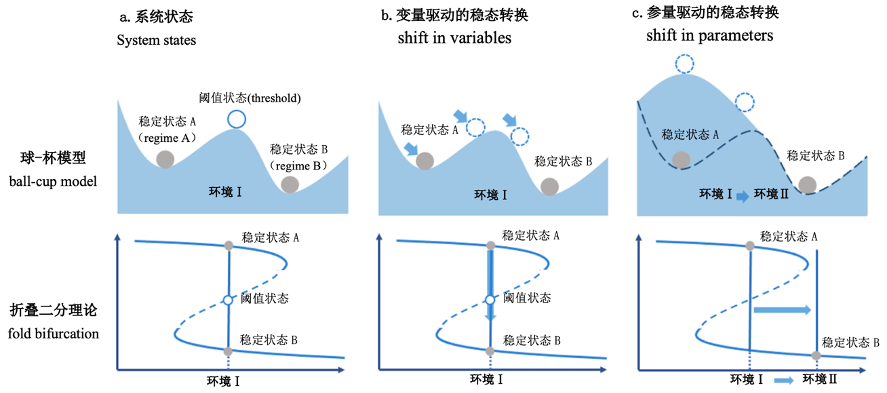
\includegraphics[width=\textwidth]{img/ch2/ch2_regime_shift.png}
    \caption[球-杯模型和折叠分岔理论对系统稳态转换的描述]{球-杯模型和折叠分岔理论对系统稳态转换的描述。
    假设系统中最多可能有2个稳定平衡状态,即稳定状态A(regime A)和稳定状态B(regime B)和1个阈值状态(threshold):
    a)环境Ⅰ条件下,球-杯模型(ball-cup model)和折叠二分理论(fold bifurcation)对系统各种状态的表征。
    b)系统稳态转换过程。变量驱动的稳态转换(shift in variables):环境Ⅰ不变时,处于稳定状态A的系统在干扰下自身突破阈值状态转换为稳定状态B。
    c)参量驱动的稳态转换(shift in parameters)。环境Ⅰ变为Ⅱ,迫使处于稳定平衡状态A的系统向新环境下仅存的稳定平衡状态B转换。(改自文献[7],[8])}
    \label{ch2:fig:regime_shift}
\end{figure}

% 地理学报
流域社会-生态系统的另一类常见人为干扰是水治理措施,但它不同于持续增加的人为压力,单独某个治理举措为稳态“小球”所施加的力也许是过小或过大的,且力的作用方向常常是不确定的,对于这类驱动力何时触发稳态转换需要“稳态循环”加以理解。
在每个稳态内的不同尺度下,社会-生态系统会自发历经开发(Growth)、保护(Senescence)、释放(Collapse)、更新(Renewal)四阶段的适应性循环[63],也有学者根据该循环将社会-生态系统框架下的治理总结为涌现(Emergence)、制度化(Institution)、更新(Renewal)三阶段(Chaffin and Gunderson, 2016)。
由于建立适应性治理体系是希望社会-生态系统状态维持在社会所需范围内,因此会产生“主动改变不良的社会-生态系统状态”与“调节并维持良好的社会-生态系统状态”两种不同的需要,通常这也是治理系统运作的主要思路。
转型治理关注社会-生态系统社会-生态系统的释放和更新阶段,强调适应性治理的实现,以及主动促使社会-生态系统完成状态的更新[64];协作治理则强调适应性治理制度化过程,旨在通过利益相关者间自组织的协作模式来实现社会-生态系统的开发与保护[65]。
转型治理企图通过自上而下的政策干预,积极将多尺度社会-生态系统转向所期待的状态[64];而协作治理的实现则常通过自下而上的手段,强调协作网络与协商制度的设计,从而建立具适应性的协作机制[68-70]。
无论自上而下或自下而上,治理流域系统产生的驱动力都既可能成为维持稳态的原因,也可能成为稳态转换的触发因素,需在分析其机制时应加以甄别。

\begin{figure}[htb] % use float package if you want it here
    \centering
    
\includegraphics{hello}
    \caption[社会-生态系统状态循环]{社会-生态系统状态循环与转型治理、协作治理的关系
    Fig.4  The relationship between social-ecological system adaptive cycle and transition / collaborative governance
    ①SES状态循环包括:开发阶段r,保护阶段K,释放阶段Ω,更新阶段α;图中展示旧的SES因转型治理而进入新的状态循环,并因协作治理的实现而延长开发保护阶段的过程;②转型治理可受其它尺度SES的影响[64,66];③协作治理的主要实现过程包括F-F-D(Face to Face Dialogue, 当面沟通),T-B(Trust-Building, 建立信任),C-P(Commitment to Process, 过程承诺),S-U(Shared Understanding, 信息对称),I-O(Intermediate Outcomes, 阶段成果)五步骤的循环[65,68,58]。}
    \label{fig:xfig0}
\end{figure}

\subsection{识别流域人水关系的稳态转换}

% 宋嘉熙 的 地理学报
在社会-生态系统稳态转换实证研究中,需从关键要素的改变切入以识别稳态转换发生,主要思路包括:辨识系统互馈变量的趋势突变、识别其它解释变量变化轨迹的不连续性、检测系统结构-功能指标的变化信号等。尽管定量识别稳态转换发生的方法、指标和标准不断提出和改进,但理解并阐明转换过程仍需要对关键要素(驱动、现象、效应)的连贯分析。本文总结了稳态转换研究中三种常见的分析路径,以黄河流域为例,结合黄河流域稳态转换研究的典型实证研究案例,阐明了三条常见分析路径。黄河流域长时间被人类活动强烈影响[48],社会-生态系统互馈关系复杂且经历了多次稳态转换,是稳态转换研究的代表性区域。

% 地理学报
此处借助“三明治”概念框图梳理其发展模式(图5)。
% 面a内是通过相互作用形成的社会网络,节点越大表明社会资本越大;面c为社会-生态系统状态集合面,其中当前状态正受到FSES的盆地吸引力。制定规则将改变社会网络结构及其对社会-生态系统的作用力,并通过路径α与路径β实现人与环境的动态适应。假设平面b为理论管理决策,韧性管理理论表明,通过设立规则(如图5:B1, B2, B3)作用于社会-生态系统(如图5:Fc1, Fc2, Fc3)从而调节系统状态是可能的[46]。但传统的管理规则相对独立,看似凌驾于社会与自然之上,实则常常失效或偏离[31]。自组织的管理思路则指出,社会网络(面a)的相互作用能够调节规则(如图5:建立Fb1, Fb2, Fb3)使其更加行之有效,且能随社会网络的变化而自适应调节。治理的理念则指出面a上的社会网络能够形成协作的组织结构,使各利益相关者都能影响规则但又不能独自左右规则[24],有利于实现自组织与适应性治理,其中根据治理目标的不同,协作治理强调维持系统状态(如图5:SES),而转型治理强调将社会-生态系统调整至更符合需求的状态(如图5:SES’)。综上所述,适应性治理理论提供了实现社会-生态系统可持续性的综合途径:从社会驱动力开始(面a),自组织并调节的管理规则(面b),进而调节社会-生态系统状态(面c);而通过适应性治理提升适应能力,旨在提升动态系统(曲面a、b通过α-β自适应)的韧性。因此,在环境变化背景下,适应性治理具有应对社会-生态系统复杂性和不确定性的潜力。

